\documentclass[border=0pt]{standalone}
\usepackage{graphicx}
\usepackage{tikz}
\usepackage{xcolor}

\definecolor{linear}{HTML}{6B7280}
\definecolor{fuxi}{HTML}{1F77B4}
\definecolor{modafno}{HTML}{17BECF}
\definecolor{sdyff}{HTML}{9467BD}
\definecolor{pixelattn}{HTML}{2CA02C}
\definecolor{dcae}{HTML}{FF7F0E}
\definecolor{bridge}{HTML}{D62728}

\newcommand{\legenditem}[3]{%
  \tikz[baseline=-0.55ex]\draw[#1,line width=#2] (0,0)--(0.52,0);%
  \hspace{3pt}#3%
}

\begin{document}
\begin{minipage}{1031.66pt}
\centering
\begin{tikzpicture}
\node[inner sep=0] (plot) {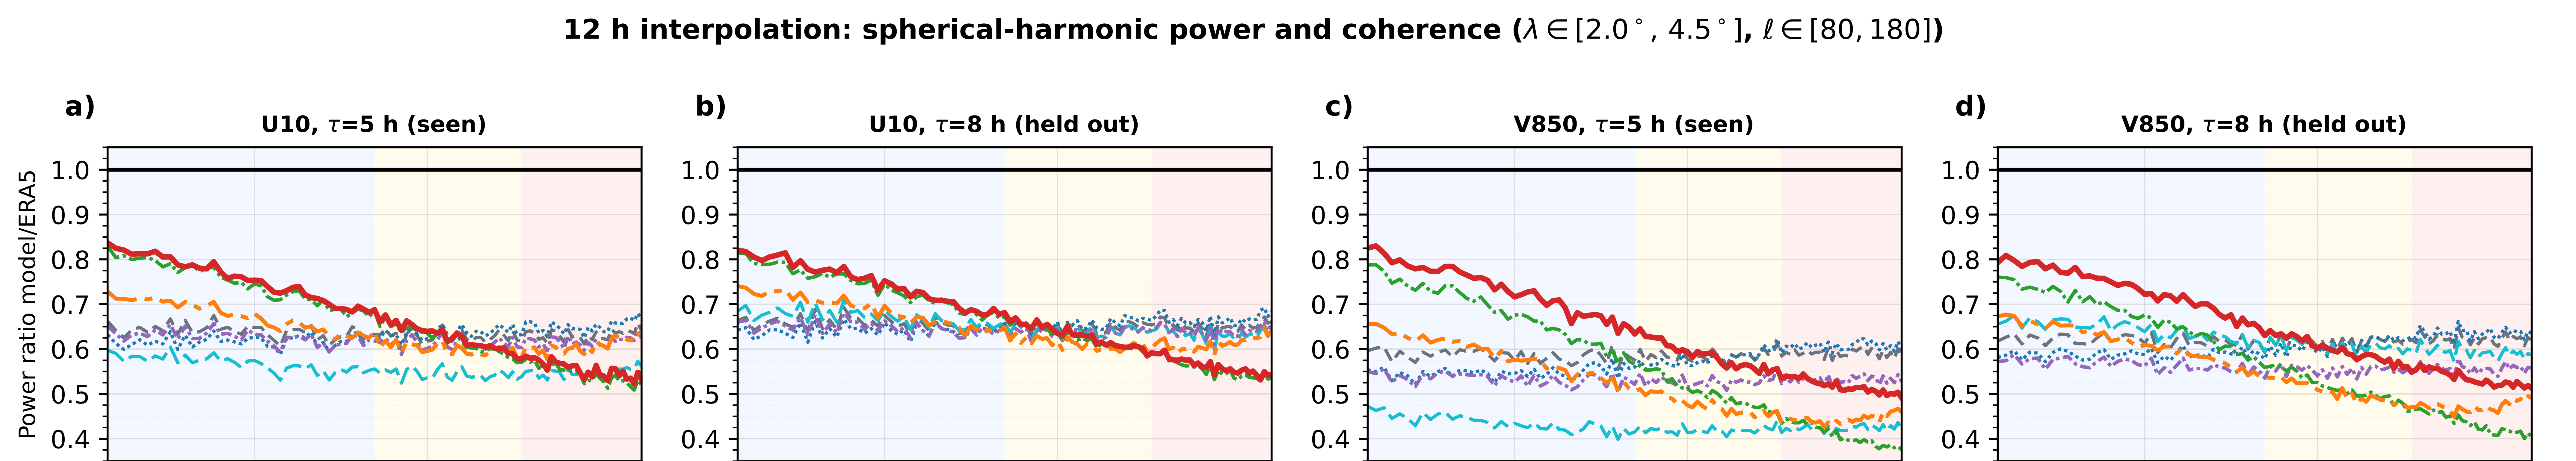
\includegraphics[
  width=\linewidth
]{images/fig_spectra_power_panels_600dpi.png}};
\fill[white] (plot.north west) rectangle
  ([yshift=-22pt]plot.north east);
\node[anchor=north,font=\bfseries\Large,yshift=-3pt] at (plot.north)
  {12 h interpolation: spherical-harmonic power retention
   ($\lambda\in[2.0^\circ,4.5^\circ]$, $\ell\in[80,180]$)};
\end{tikzpicture}\\[-1pt]
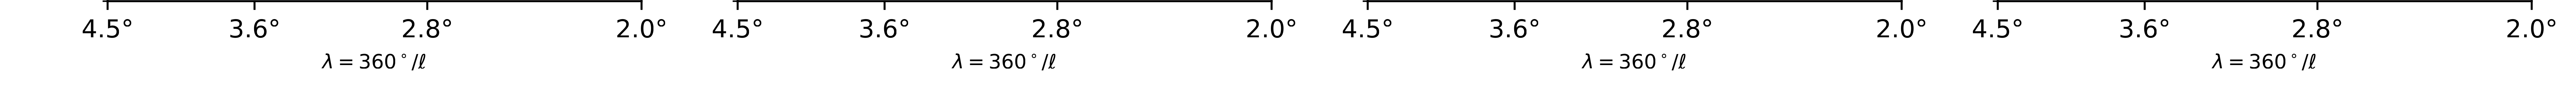
\includegraphics[
  width=\linewidth
]{images/fig_spectra_power_axis_600dpi.png}\\[5pt]
\small
\begin{tabular}{@{}llll@{}}
\legenditem{linear,dashed}{0.8pt}{Linear Interp.} &
\legenditem{fuxi,densely dotted}{0.8pt}{SwinV2} &
\legenditem{modafno,dashed}{0.8pt}{ModAFNO} &
\legenditem{sdyff,dash pattern=on 3pt off 1pt on 1pt off 1pt}{0.8pt}{S-DYff} \\[4pt]
\legenditem{pixelattn,dash pattern=on 5pt off 1pt on 1pt off 1pt}{0.8pt}{PixelAttn-VFI} &
\legenditem{dcae,dashed}{0.8pt}{WeatherDCAE-14M} &
\legenditem{bridge}{1.5pt}{WeatherBridge} &
{}
\end{tabular}
\end{minipage}
\end{document}
